\chapter{Generatore di Lehmer}
	\label{cap:generatorerandom}

Il progetto si pone di testare il noto generatore pseudo-casuale di numeri 
random di Lehmer utilizzando, a tale scopo, uno dei test di casualit\'a 
illustrati nel libro \textit{Discrete-Event Simulation: A first course}.
All'interno del progetto si \'e scelto di utilizzare la versione del generatore
fornita come libreria C dallo stesso libro, \'e stato quindi creato un programma C
che si interfaccia con tali librerie, tramite chiamate alle API della libreria 
stessa,
che serva a testare la effettiva correttezza di tale implementazione.
Al fine di comprendere al meglio i risultati ottenuti verranno anche
presentati dei grafici riassuntivi del test effettuato.

\section{Funzionamento}
Il \textit{generatore di Lehmer} \'e un generatore basato su un algoritmo che da 
origine ad una sequenza di numeri pseudo-casuali. \'E definito da due parametri:

\begin{itemize}
 \item un modulo \textbf{\textit{m}}, che \'e un numero primo molto grande (in 
questo caso la libreria usa $2^{31} - 1$);
 \item un moltiplicatore \textbf{\textit{a}} che rappresenta un numero intero 
compreso tra 1 ed m-1.
\end{itemize}

\noindent La sequenza numerica pseudo-random viene generata tramite la formula :

\begin{center} $x_{i+1} = ax_{i} mod m$ \end{center}

\noindent Questa sequenza parte da un numero $x_{0}$ detto seed, anch'esso 
scelto tra 1 ed m - 1. Non tutte le combinazioni di a ed m però sono ottimali 
per realizzare una sequenza di numeri che garantiscano una buona randomicit\`a. 
Per verificare dunque se un seed e un moltiplicatore garantiscono un buon 
livello di 
randomicit\`a esistono dei test empirici, nel capitolo successivo tale generatore 
verr\`a sottoposto ad uno di questi.

\section{Test degli estremi}
Il test scelto per effettuare la verifica sul generatore, con parametri:
\begin{center}
$(a,m) = (48271, 2^{31} - 1)$
\end{center}

\noindent \'e conosciuto come ``\textit{Test degli estremi}''. 
Per la simulazione di tale test si pu\`o riassumere il processo in tre passi:
\begin{itemize}
 \item Generazione di un campione di valori con chiamate ripetute al generatore
 \item Computazione di un test statistico la cui distribuzione (pdf o funzione 
di densit\`a di probabilit\`a) \'e nota su variabili random uniformi in (0,1) indipendenti e identicamente 
distribuiti
 \item Valutare la verosimiglianza del valore computato del test statistico con 
la relativa distribuzione
 teorica da cui \'e stato assunto adottando una metrica basata sulla distanza 
lineare
\end{itemize}

Questo test si basa sulla seguente considerazione:

\vspace{0.5cm} \noindent \textbf{Teorema} Se $U_{0}^{}$, 
$U_{1}^{}$,...,$U_{d-1}^{}$ \'e una sequenza di variabili \textit{Uniform(0,1)} e 
se 

\begin{center}R = max{$U_{0}^{}$, $U_{1}^{}$,...,$U_{d-1}^{}$} \end{center} 

\noindent allora la variabile U = $R_{}^{d}$ \'e una \textit{Uniform(0,1)} 
\footnote{Attenzione: il teorema afferma che la variabile U \'e una Uniform(0,1), 
mentre la variabile R non lo \'e.}.

In pratica tale test verifica che la variabilit\`a delle altezze dell'istogramma 
prodotto dai numeri pseudo-casuali generati \'e sufficientemente piccola da poter 
concludere che questi numeri appartengano ad una popolazione 
\textit{Uniform(0,1)}. Questa operazione \'e fondamentale in quanto tutte le 
altre distribuzioni di probabilit\`a contenute all'interno della libreria 
utilizzata vengono generate a partire dalla \textit{Uniform(0,1)}.

\section{Algoritmo}
L'algoritmo del test degli estremi effettua un raggruppamento (batching) dei 
valori estratti dal generatore in gruppi di uguale lunghezza (determinato dal 
parametro d), trovando il 
massimo di ogni batch, elevando tale massimo all d-esima potenza e conteggiando 
tutti i massimi generati in un array. Tale funzione viene applicata per ogni 
stream el generatore Lehmer.
Tutto ci\`o \'e illustrato di seguito:
\begin{verbatim}
  for(stream = 0; stream < 256L; stream++) {
      long o[K];
      memset(o, 0, K * sizeof(long));
      for(i = 0; i < N; i++) {
          double r = Random();
          for(j = 1; j < D; j++) {
              u = Random();
              if(u > r) r = u;
          }
          u = exp(D * log(r));
          x = u * K;
          o[x] ++;
      }
  }
\end{verbatim}
Per ogni stream, si determina quindi la variabile chi-quadro v tramite questa 
funzione:
\begin{verbatim}
      for(i = 0; i < K; i++) {
	      v += (square(o[i] - e_x));
      }
      v /= e_x;
\end{verbatim}

I valori critici v*1 e v*2 vengono calcolate utilizzando la funzione inversa 
\textit{idfChisquare(long n, double u)}  fornita dalla libreria rvms.c del libro di 
testo. Bisogna precisare che per il calcolo 
di tali variabili statistiche \'e stato scelto un livello di confidenza con 
parametro alpha = 0.05, mentre i parametri N e K sono rispettivamente N = 100000 
e K = N/20 = 5000.
Successivamente si confronta la statistica chi quadro v, determinata al passo 
precedente, con i valori critici  v*1 e v*2 , per ogni stream (in totale sono 256 
variabili chi-quadro v ).
Se $v < v*1 o v > v*2$ il test fallisce (per quello stream) con probabilità 1 - 
alpha.

\section{Test e conclusioni}
\noindent Il grafico risultante di questo test empirico \'e illustrato di seguito:

\begin{figure}[H]
 \begin{center}
  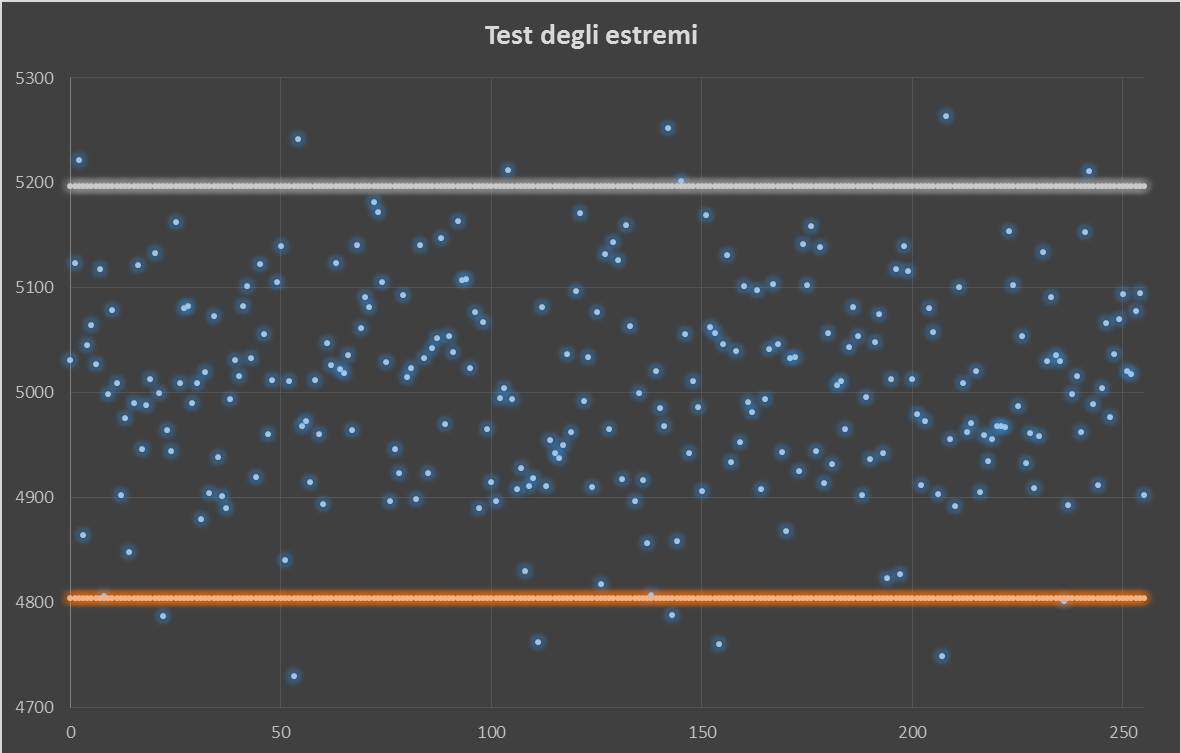
\includegraphics[scale=0.45]{img/test.png}
  \caption[Test degli estremi]{Test degli estremi}
  \end{center}
\end{figure}

\vspace{0.5cm}
I valori critici sono visualizzati come linee orizzontali: quella inferiore rappresenta
v*1 = 4804.92 mentre quella superiore è v*2 = 5196.86

Dalla simulazione effettuata si \'e notato che il numero di test statistici $v > v*2$ sono stati 7 
esattamente come il numero di test $v < v*1$. Di seguito \'e riportato l’output del programma:

\begin{figure}[H]
  \begin{center}
  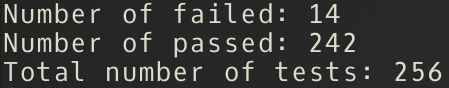
\includegraphics[scale=0.7]{img/test_estremi.png}
  \caption[Risultati]{Risultati}
  \end{center}
\end{figure}


Considerando il numero totale di test falliti (upper e lower bound) pari a 14, si nota che non
ci si discosta molto rispetto al valore atteso approssimato; infatti in 256 test con un livello di
confidenza del 95\% il valore aspettato è circa 256 * 0.05 = 13 fallimenti. Questo valore pu\`o 
essere una indicazione della bont\`a del generatore di Lehmer implementato.
